\documentclass[12pt,a4paper]{article}
\usepackage{graphicx}
\usepackage[toc,page]{appendix}
\usepackage{xcolor}
\usepackage{listings}
\lstset{basicstyle=\ttfamily,
  showstringspaces=false,
  commentstyle=\color{red},
  keywordstyle=\color{blue}
}


\begin{document}
\begin{titlepage}
	\centering
	
\includegraphics[width=0.55\textwidth]{tentacle.png}\par\vspace{1cm}
	{\scshape\LARGE Smart Soft-Robotics Tentacle Documentation\par}
	\vspace{1cm}
	{\scshape\Large NoodleBot\par}
	\vspace{1.5cm}
	{\itshape \textbf{Byron Becker, Surjith Singh, Vidur Sarin, Adam Seifkas, Stan James, Ryan Riley}\par}
	{\large \today\par}
\end{titlepage}

\tableofcontents

\newpage
\section{Introduction}

The NoodleBot team is creating a robot tentacle from a pool noodle, para cord, stepper motors, a micro controller, and machine learning software. The device is intended for those with accessibility concerns and will allow those with a limited range of motion to reach out and potentially manipulate objects.

\section{Overview}


\section{Hardware}

Our first concern was creating the physical device

\section{Software}

\subsection{Software Overview}

\begin{figure}[h!]
\centering
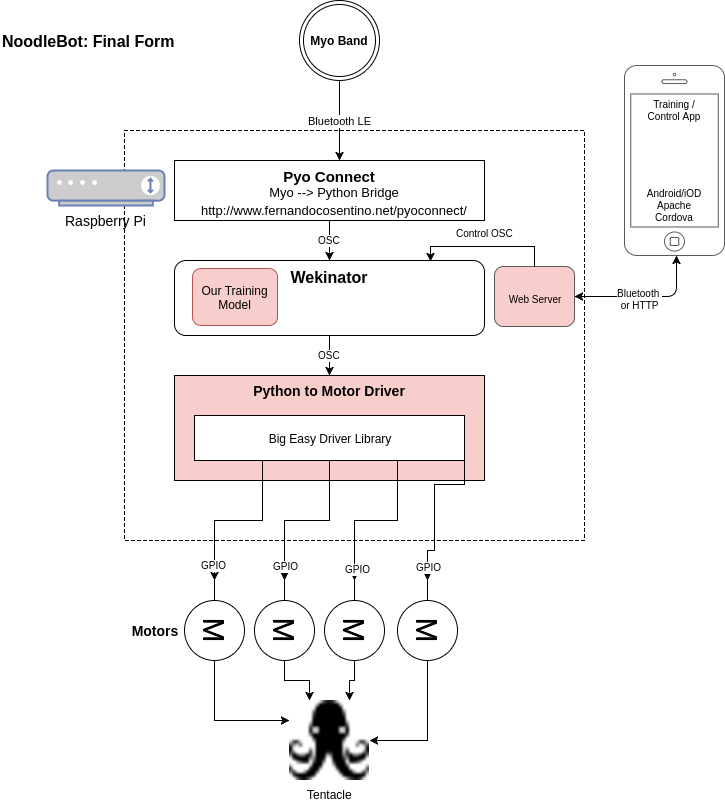
\includegraphics[width=0.55\textwidth]{SoftwareFlow.png}\par\vspace{1cm}
\caption{Software Flow}
\label{fig:flow}
\end{figure}

\subsection{Myo Osc and Related Python Scripts}

\subsection{Mobile App}


The project includes a Mobile App which is to be used as a remote control of the training and running process occurring on the Raspberry Pi. Having this functionality allows the entire project to be mobile and not reliant on a laptop or desktop system. The app cross-platform: both iOS and android are supported. 

\subsection{Machine Learning with Wekinator}

\subsection{Hardware Control Code}

The control code consists of several python programs created to run on the Raspberry pi. It accepts OSC messages of 4 values, and will then have the 4 stepper motors (A,B,C,D) try to move to those positions. "Position" is defined as steps away from the initial point where motors begin, either positive or negative. So if steppers are currently at positions [10.0, 0.0, 6.0, 0.0], then an OSC messages of [1.0,-2.0,5.0,0.0] will have stepper A move 9 steps counter-clockwise, stepper B move two steps counter-clockwise, stepper C move 1 step clockwise, and stepper D does nothing.

\paragraph{- `TentacleControl.py` :} Creates OSC server, creates our 4 steppers, and starts them updating
\paragraph{- `Stepper.py` :} Our tentacle-specific implementation of stepper. Handles bookkeeping of current stepper position, periodic updates (in own thread)
\paragraph{- `Easydriver.py` :} Copy of existing github code that provides basic functionality to steppers via easydriver.

As of now its hard coded that motors move only one step per update cycle.

\paragraph{Settings}
\hfill \break
Constants in the code can be modified to set how often the steppers update their position, OSC server address, and other settings.

\hfill \break
Enable/Disable steppers by commenting lines 36-40 in TentacleControl.py
\hfill \break \hfill \break
$stepper{\_}time{\_}interval{\_}seconds = 0.25-$ Steppers will continually update their position on this schedule and attempt to move toward the last-set goal position, no matter how many OSC messages are received.
\hfill \break \hfill \break
Stepper minimum/maxium in Stepper.py



\paragraph{Running}

\begin{lstlisting}

To run:
    python TentacleControl.py

To test:
 - Run wekinator with 4 outputs.
 - Modify outputs to have range equal to steps of motion desired. (e.g. -40.0 to +40.0)
 - Move sliders
 \end{lstlisting}

\hfill \break
Note: `Stepper.py` will detect if you are running on Raspberry Pi, and will use a stub file if you are *not*. This will show the same debug messages as real code, but (obviously) won't do anything with GPIO.

\hfill \break
Sample output: 
\begin{lstlisting}

	$ python TentacleControl.py
	Could not find RPi module. So using stub GPIO module.
	New stepper created: Stepper A
	      [ENB|MS1|MS2|MS3|RST|SLP|STP|DIR]
	Pins: [  4|  5|  6|  7|  0|  0|  3|  2]
	New stepper created: Stepper B
	      [ENB|MS1|MS2|MS3|RST|SLP|STP|DIR]
	Pins: [ 10| 11| 12| 13|  0|  0|  9|  8]
	New stepper created: Stepper C
	      [ENB|MS1|MS2|MS3|RST|SLP|STP|DIR]
	Pins: [ 16| 17| 18| 19|  0|  0| 15| 14]
	New stepper created: Stepper D
	      [ENB|MS1|MS2|MS3|RST|SLP|STP|DIR]
	Pins: [ 22| 23| 24| 25|  0|  0| 21| 20]
	Created 4 steppers
	Tentacle Control is listening for OSC message /wek/outputs, ip 127.0.0.1 port 12000
	0.0934-Stepper A	In goal position: 0.00
	0.0940-Stepper A	In goal position: 0.00
	0.0946-Stepper A	In goal position: 0.00
	0.0953-Stepper A	In goal position: 0.00
	0.0959-Stepper A	In goal position: 0.00
	0.0965-Stepper A	In goal position: 0.00

\end{lstlisting}
\section{Challenges}

\section{Future Work}



\end{document}
